\chapter{The Models Manager}

The model manager tab in the GUI provides the functionality to create models of various types, configure them, specify the variables to use in them, and then estimate their parameters if they have a form that needs to be estimated -- such as regression models or discrete choice models.  A more thorough description of the types of models that can be implemented in OPUS is provided in Chapter \ref{chap:creating-models}.

\begin{figure}[htp]
\begin{center}
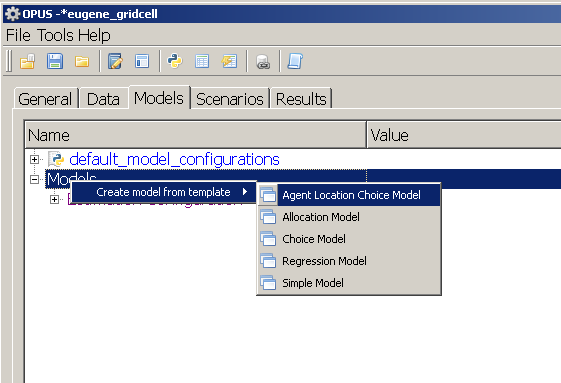
\includegraphics[scale=0.6]{part-gui/images/model-manager-create-model-from-template.png}
\end{center}
\caption{Creating a New Model from a Template}
\label{fig:create-model}
\end{figure}

\section{Creating an Allocation Model}

To demonstrate the creation of an Allocation Model in Opus, let us assume that the task at hand is to create a model that allocates home-based jobs to zones.  Home-based jobs are those jobs that are located in properties that are residential in character.  Assume that we have no behavioral information about this problem, other than the insight that home-based jobs are... home-based.  So we can infer that we should probably allocate these jobs to places that have housing (or households).  In allocating these jobs to zones (traffic analysis zones used in the travel model), we can count how many residential units are in each zone, and use this as the weight to allocate the total home-based jobs to zones.  That is, we want to proportionately allocate home-based jobs to zones, weighted by the number of residential units in the zone.  This is equivalent to saying that we want each residential unit to have an equal probability of receiving a home-based job (assuming that we do not have any information to suggest which residential units would be more likely than others to receive such a job).

The next consideration is the capacity of zones to absorb home-based jobs.  One simplifying assumption we could make is that there is a maximum of one home-based job per residential unit in a zone.  On average, our aggregate information suggests that most residential units do not have a home-based job, so this assumtion should not be constraining.

We now have all the information we need to specify a model for home-based jobs.  We will name the model allocate\_home\_based\_jobs, to be descriptive.  The table below contains the \emph{arguments} we will need to use in creating this model in the GUI.

\begin{table}[htp]
\caption{Creating an Allocate Home Based Jobs Model}
\label{tab:allocation-model}
\begin{center}
\begin{tabular}{ p{1.5in}  p{4.4in}  }
\toprule[1.5pt]
Configuration Entry & Value \\
\midrule
Model Name & allocate\_home\_based\_jobs\_model \\
Dataset & zone \\
Outcome Attribute & home\_based\_jobs \\
Weight Attribute & zone.aggregate(building.residential\_units) \\
Control Totals & annual\_employment\_control\_totals \\
Year Attribute & year \\
Capacity Attribute & zone.aggregate(building.residential\_units) \\
\bottomrule
\end{tabular}
\end{center}
\end{table}

The capacity to create new allocation models, such as this, is now available in the Opus GUI.  To create this allocation model, or one like it, open a project, like seattle\_parcel, and go to the Model Manager tab.  Open model\_system, and you will see an \emph{allocation\_model\_template}.  Right-click on this and select \emph{Add to current project}, then right-click again and select \emph{Copy Node}.  Assign the name \emph{allocate\_home\_based\_jobs\_model} when prompted for the XML Node Name to create.  Now, edit the values in the run arguments of the newly created node (at the bottom of the models list) to match the values in the table above. Figures \ref{fig:model-allocation-1} and \ref{fig:model-allocation-2} show screenshots of these initial steps in this process.  Figure \ref{fig:model-allocation-1} shows the model template for an allocation model, with fields identified as needing to be filled in by the user. Figure \ref{fig:model-allocation-2} shows the new copy, named and filled in with the actual settings, from the table above. 

\begin{figure}[htp]
\begin{center}
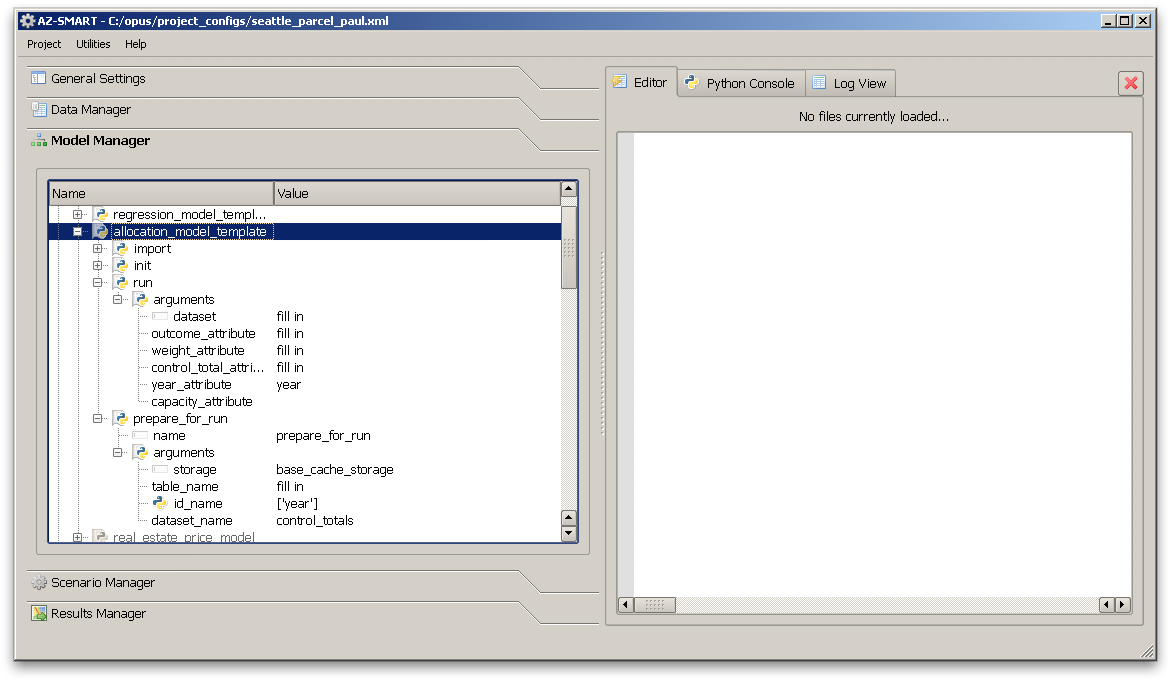
\includegraphics[scale=0.35]{graphics/create-model-template-allocation.png}
\end{center}
\caption{Template for Allocation Model}
\label{fig:model-allocation-1}
\end{figure}

\begin{figure}[htp]
\begin{center}
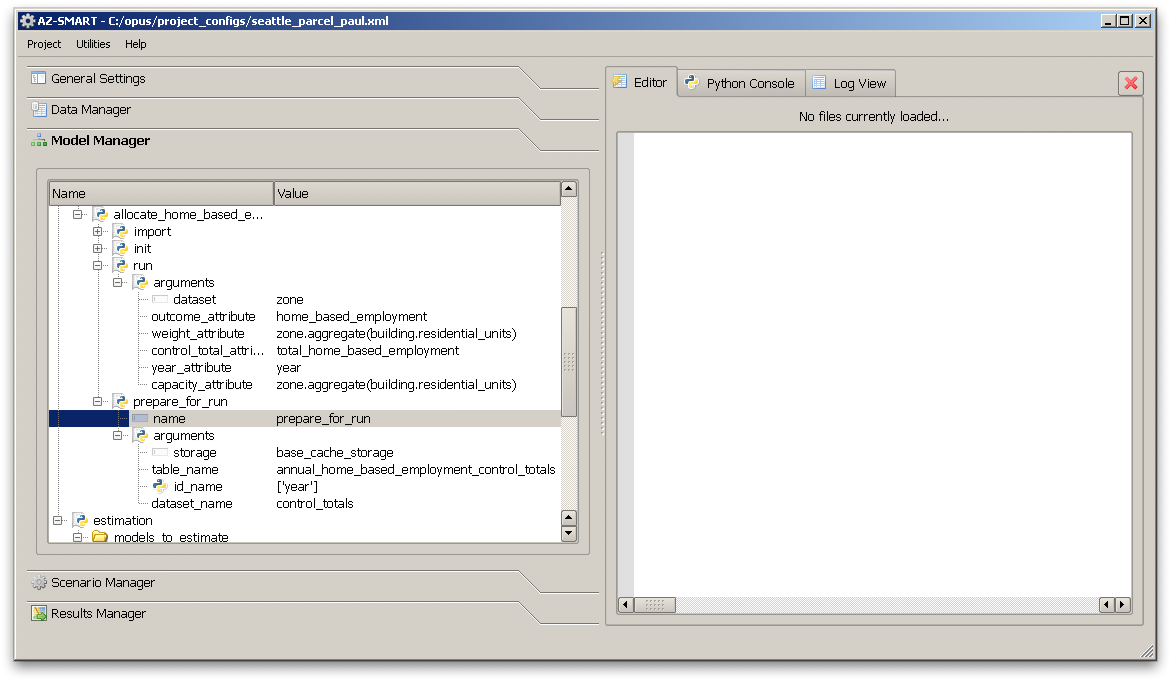
\includegraphics[scale=0.35]{graphics/create-allocation-model.png}
\end{center}
\caption{Creating Home-Based Employment Allocation Model}
\label{fig:model-allocation-2}
\end{figure}

Now the new allocation model exists.  It will still need to be added to a list of models to run in order to actually be executed.  This is done in the Scenario Manager.  Select the models\_to\_run entry under the Seattle\_baseline, and if it is not already editable, right-click and select Add to current project.  Then right-click and select Copy Node, and assign the new model name to it.  For testing purposes, it would be advisable to change the values of all the other models to Skip, and just run the one new model to test it.   After this, you should be able to right-click on the scenario name in the GUI and run the scenario, with the new model actually executing.  This is shown in the screenshot in Figure \ref{fig:model-allocation-3}.

\begin{figure}[htp]
\begin{center}
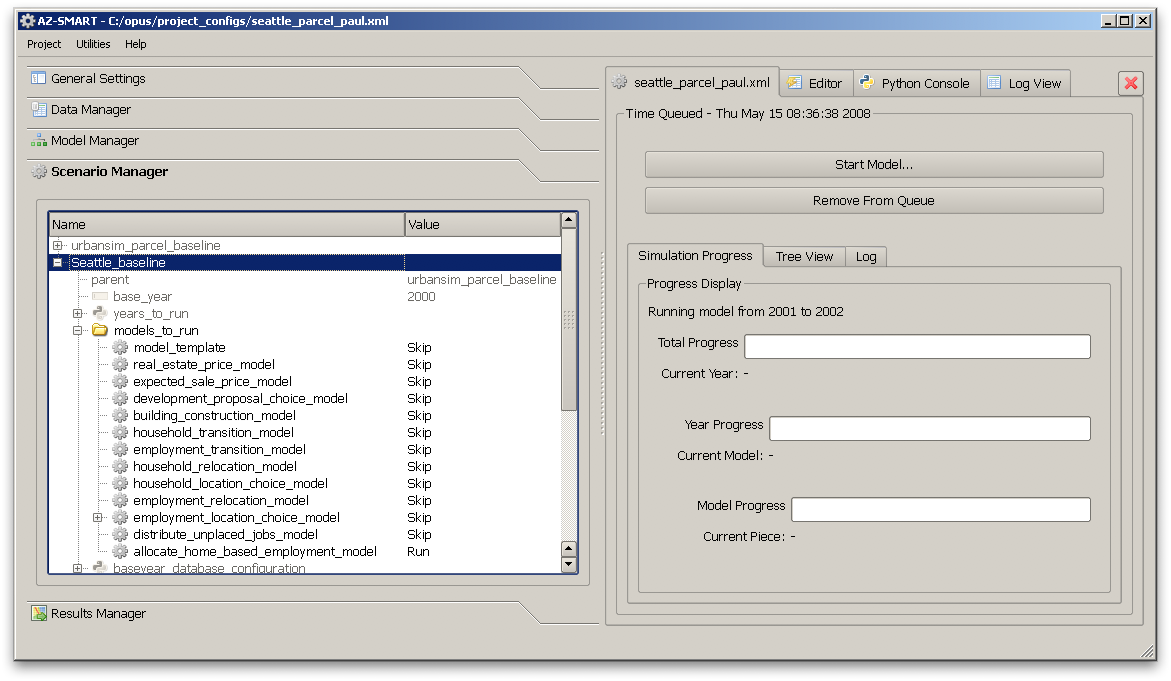
\includegraphics[scale=0.35]{graphics/create-allocation-model-run.png}
\end{center}
\caption{Running the Home-Based Employment Allocation Model}
\label{fig:model-allocation-3}
\end{figure}

More advanced data handling and preparation is also available for this class of model.  A specific set of extensions has been added for the Maricopa Association of Governments to allow the control totals to be stored in an Excel spreadsheet, and the weight and capacity attributes to be stored in an ESRI Shape file or geodatabase.  These extensions are currently handled in the \emph{prepare for run} method of the model, in Python code, and is not directly available in the GUI.

\section{Creating a Regression Model}

Regression models are simple to specify in the Opus GUI, and can be estimated and simulated within the graphical interface.  We will use as an example the development of a model to predict land values per square foot for all parcels.  Assume we want to create a model that predicts the value of land, per square foot, using the tax assessor valuations of land value and the square footage measures of each parcel available in the assessor data.  Since the outcome is continuous, but truncated at zero and increasing to quite large values, we might want to use a log-transformation of the price per square foot.  This would allow for representing the diminishing returns to larger quantities on some attributes.  We begin, however, with a simple nominal value per square foot, which implies that a unit increase in the amount of an independent variable, adds a constant dollar amount to the value of land per square foot.

The table below summarizes the arguments we would set for creating this model:

\begin{table}[htp]
\caption{Creating a Land Price per Square Foot Model}
\label{tab:land-price-sqft-model}
\begin{center}
\begin{tabular}{ p{1.3in}  p{1.3in} p{3.0in}  }
\toprule[1.5pt]
Configuration Entry & Node & Value \\
\midrule
Model Name & & land\_price\_sqft\_model \\
Dataset & Run and Estimate & parcel \\
Specification Table & Prepare for Run & land\_price\_sqft\_model\_specifications \\
Coefficients Table & Prepare for Run & land\_price\_sqft\_model\_coefficients \\
Outcome Attribute & Estimate &ln\_price\_sqft = \\ & & ln\_bounded(parcel.land\_value/parcel.parcel\_sqft)  \\
\bottomrule
\end{tabular}
\end{center}
\end{table}

To create this model in the Opus GUI, you would first make sure that you have made the Model System editable, and then copy the regression model template to a new XML node, which we shall call in this case land\_price\_sqft\_model.  Right-click on the regression\_model\_template, and save the copy as land\_price\_sqft\_model.  Once this new model configuration is created, we need to fill in fields marked as 'fill in' in the value field.  Use the values in the table above to fill in the appropriate values to create a model to predict land values per square foot.  Figure \ref{fig:model-regression-1} shows the fields to be filled in or modified to create this model.

\begin{figure}[htp]
\begin{center}
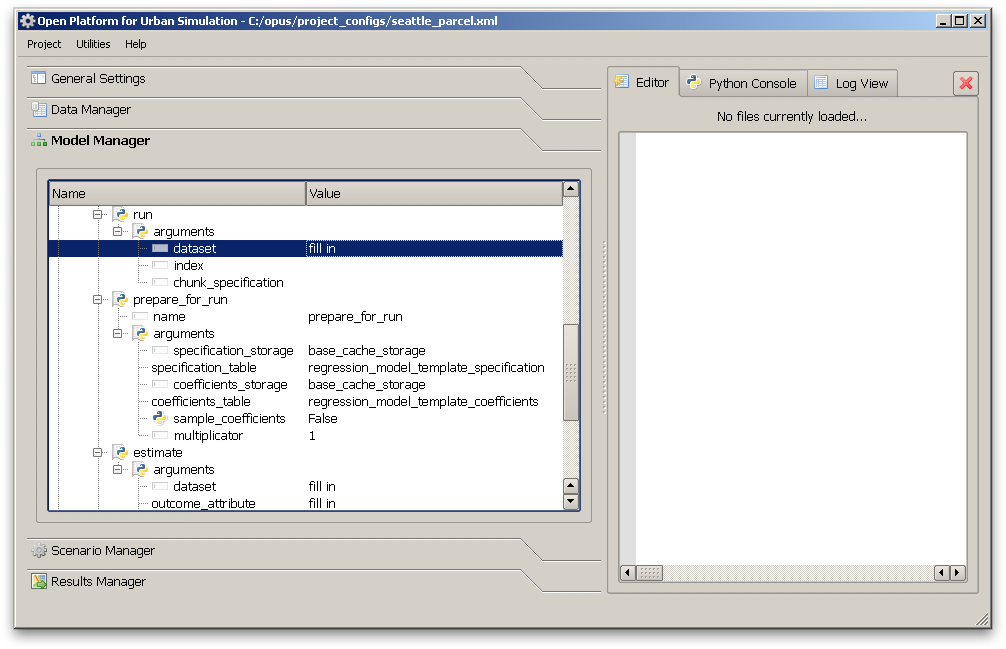
\includegraphics[scale=0.4]{graphics/create-regression-model.png}
\end{center}
\caption{Create a Regression Model from a Template}
\label{fig:model-regression-1}
\end{figure}

Once the correct values have been assigned to the configuration of the new model, we can move to the task of specifying and estimating this model.  For this, we need to move from the model system component of the GUI to the estimation node, below it.  Here again we will see a model\_template.  Copy this template to a new name, to match the name of the model we just created: land\_price\_sqft\_model.  Once this is done, we need to fill in the specification for this model.

\begin{figure}[htp]
\begin{center}
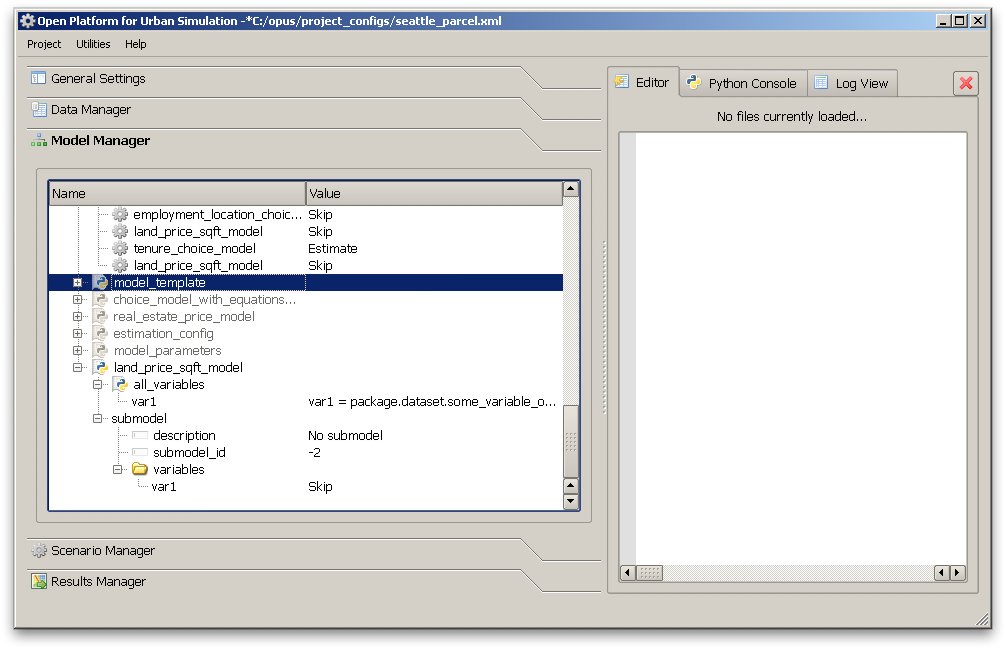
\includegraphics[scale=0.4]{graphics/specify-regression-template.png}
\end{center}
\caption{Specify a Regression Model from a Template}
\label{fig:model-regression-2}
\end{figure}

A preliminary specification for such a model might include a constant, at a minimum, since we need an intercept for a regression model in general (we don't want to force the assumption that the intercept is at zero).  We might also add, for a very simple specification, an accessibility variable like the generalized cost to the central business district of Seattle.  Another likely candidate would be distance from major highways, or a dummy variable identifying parcels that are very close to a highway.  A specification like this can be easily put into the model, in the GUI, by simply adding expressions into the all\_variables list, and then including the names of these expressions in the submodel list.  Note that if a model applies the same specification to all the data, it has no submodels, and the submodel\_id is set to -2.  We will use this default in this example.  Table \ref{tab:land-price-sqft-model-specification} shows an initial specification for this new model, creating two expressions to add to the model.


%\begin{figure}[htp]
%\begin{center}
%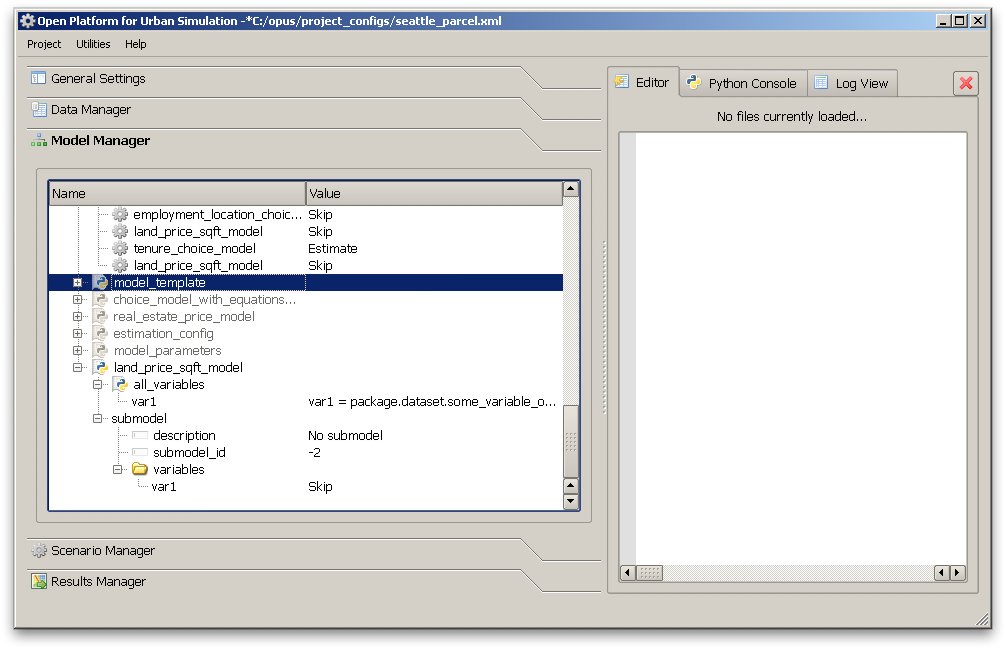
\includegraphics[scale=0.4]{graphics/specify-regression-template.png}
%\end{center}
%\caption{Land Price per Sqft Model Specification}
%\label{fig:model-regression-3}
%\end{figure}

\begin{table}[htp]
\caption{Sample Initial Specification of a Land Price per Square Foot Model}
\label{tab:land-price-sqft-model-specification}
\begin{center}
\begin{tabular}{ p{1.5in}  p{4.0in}  }
\toprule[1.5pt]
Name & Expression \\
\midrule
cbd\_time & parcel.disaggregate(zone.travel\_time\_to\_cbd)\\
hwy300 & parcel.disaggregate(gridcell.distance\_to\_highway)$<$300\\
\bottomrule
\end{tabular}
\end{center}
\end{table}


Once the model specification has been entered, we can add it to the list of models to estimate, and select it as the model to estimate.  This can be done by right-clicking on the regression model template entry in the models to estimate node, assigning the new model name to the copy, and changing its value from skip to estimate.  %The result is shown in Figure \ref{fig:model-regression-4}.

%\begin{figure}[htp]
%\begin{center}
%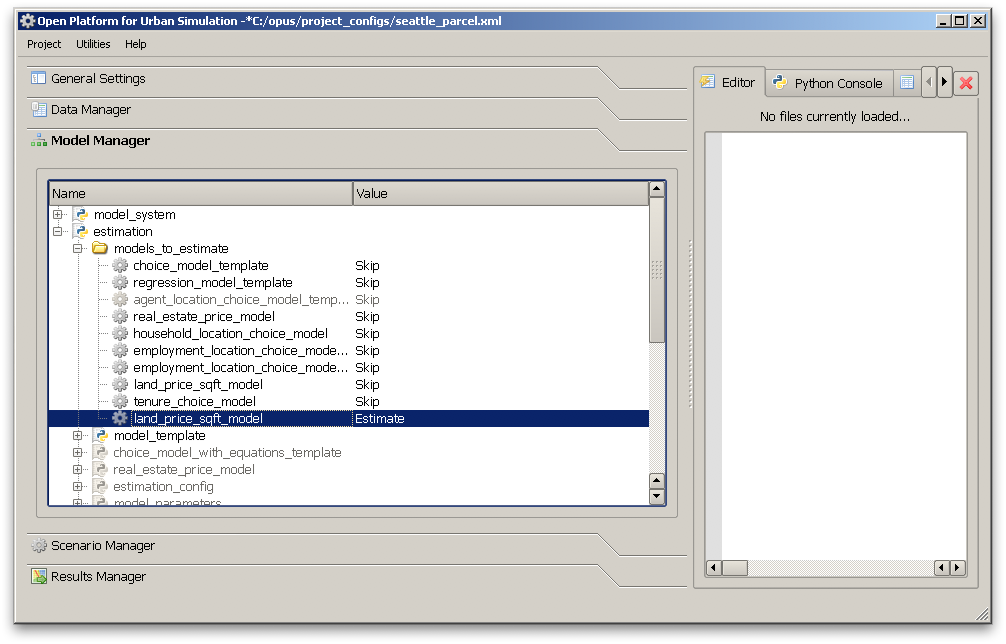
\includegraphics[scale=0.4]{graphics/add-to-models-to-estimate.png}
%\end{center}
%\caption{Adding the New Model to the List of Models to Estimate}
%\label{fig:model-regression-4}
%\end{figure}


\section{Creating a Choice Model}
The next type of model we will create is a choice model.  This is a very common modeling application, and is used widely.  Our example for this demonstration is a model of housing type choice, which for purposes of keeping the example simple, we reduce to two alternatives: single-family housing type, or other.  It is likely that households choosing to live in single-family housing may make different trade-offs in other choices, such as travel, and car ownership.  By reducing the model to two outcomes, we create a binary choice model specification.  We always need to use one alternative as a base of comparison in choice models, so for this model we will use the other housing type as the base of comparison.  

Below are the configuration settings for creating a choice model of housing type.  In order to create this model for estimation purposes, we will exclude the few households that are in non-residential property types, and only keep those in multi-family, condominium, and single-family housing.  These are reflected by building type id values of 4, 12, and 19, respectively, in the seattle parcel data.  Filtering the data to include only these three values can be done with the numpy logical\_or command, but since it takes only two arguments, we need to create a nested comparison, as shown below.  Since there are three housing types represented in this data, and we want to create a binary choice outcome for simplicity, it is necessary to create a dependent variable that is 2 if the household occupies a single family house, and 1 otherwise.  In this example, since we will use the entire household table, we draw a small sample of 5\% of the agents to use in estimating the model.

\begin{table}[htp]
\caption{Creating a Housing Type Choice Model}
\label{tab:housing-type-choice-model}
\begin{center}
\begin{tabular}{ p{1.2in}  p{1.2in} p{3.2in}  }
\toprule[1.5pt]
Configuration Entry & Node & Value \\
\midrule
Model Name & & housing\_type\_choice\_model \\
Choice Set & Init & [1, 2] \\
Choice Attribute & Init & single\_family=(household.disaggregate\\ & & (building.building\_type\_id)==19)+1 \\
Estimation Size Agents & Init.Estimation Config & 0.05 \\
Agent Set & Run, Prepare for Run, Estimate, Prepare for Estimate & household \\
Agent Filter & Prepare for Run & numpy.logical\_or(numpy.logical\_or(household.\\ & & disaggregate(building.building\_type\_id)==4,household. \\ & & disaggregate(building.building\_type\_id)==12),household.\\ & & disaggregate(building.building\_type\_id)==19) \\
Specification Table & Prepare for Run & housing\_type\_choice\_model\_specifications \\
Coefficients Table & Prepare for Run, Prepare for Estimate & housing\_type\_choice\_model\_coefficients \\
\bottomrule
\end{tabular}
\end{center}
\end{table}

Figure \ref{fig:configure-choice-model} shows the housing type choice model configuration in progress.  For a binary choice model such as this, the specification of the model is quite similar to the specification of the regression model, but there are some subtle differences.  The most important one is that, as this model is implemented in Opus now, it requires at least one variable in each equation - that is - per alternative.  We typically assign the constant to alternative 1, and all other variables to alternative 2.  In a future revision of the code, the base alternative will not take any variables (this is the more standard implementation).  Figure \ref{fig:choice-model-specification} shows the initial specification of the housing type choice model, with a constant for the other housing types, and income and has\_children included in the utility specification for the single family housing alternative. 

Once the model is specified, it needs to be added to the list of models to estimate, and selected as the model to estimate, as was the case in the preceding regression model example.  Once the model has been added and the project saved, the model can be estimated with the normal right-click option on the models to estimate node.  The results are shown in Figure \ref{fig:choice-model-estimation}.

\begin{figure}[htp]
\begin{center}
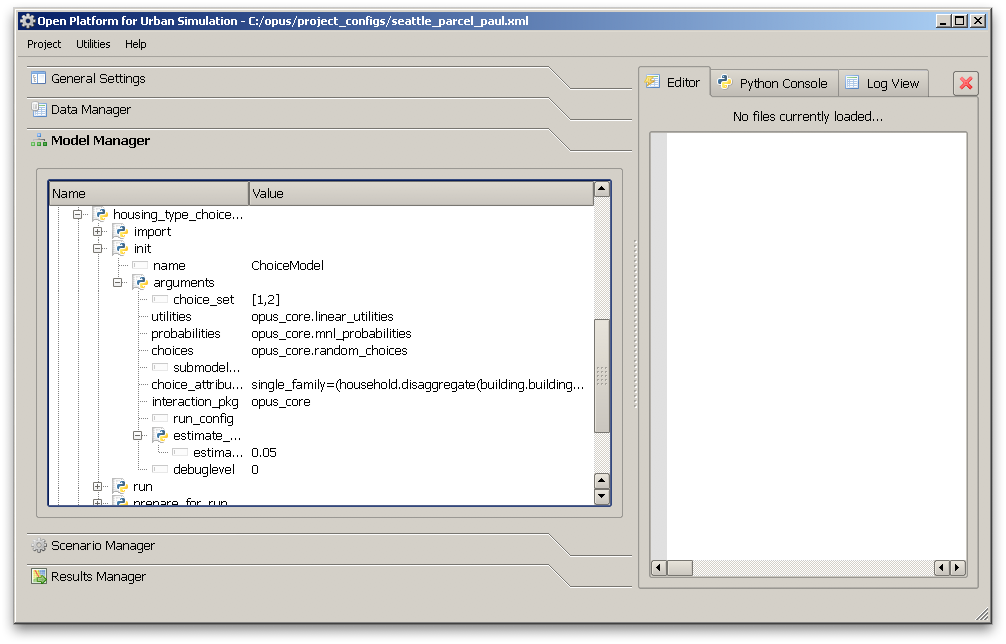
\includegraphics[scale=0.35]{graphics/configure-choice-model.png}
\end{center}
\caption{Configuring the Housing Type Choice Model}
\label{fig:configure-choice-model}
\end{figure}

\begin{figure}[htp]
\begin{center}
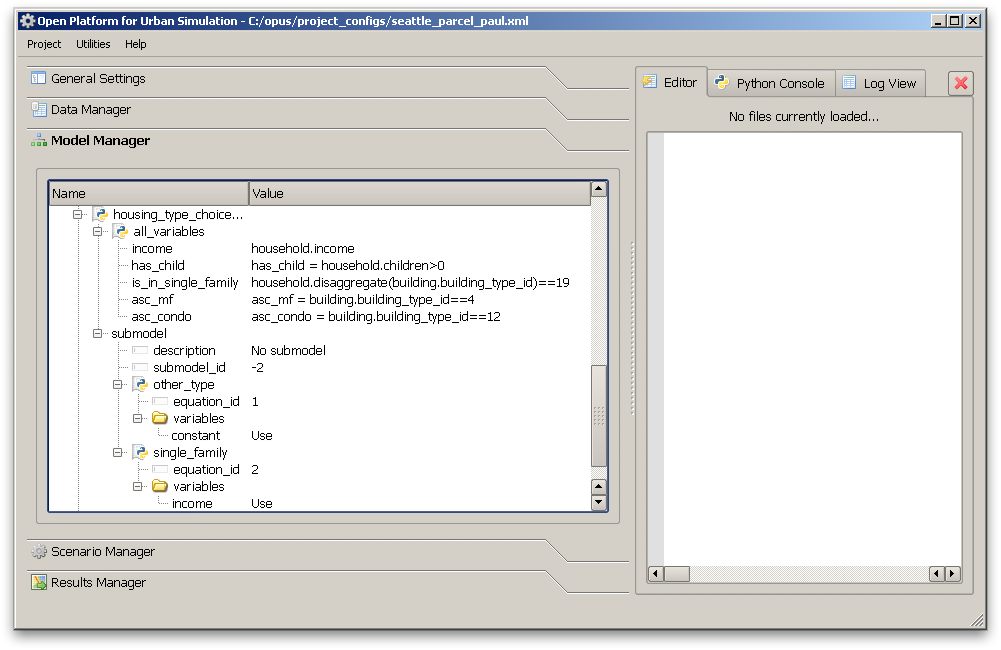
\includegraphics[scale=0.35]{graphics/choice-model-specification.png}
\end{center}
\caption{Specifying the Housing Type Choice Model}
\label{fig:choice-model-specification}
\end{figure}

\begin{figure}[htp]
\begin{center}
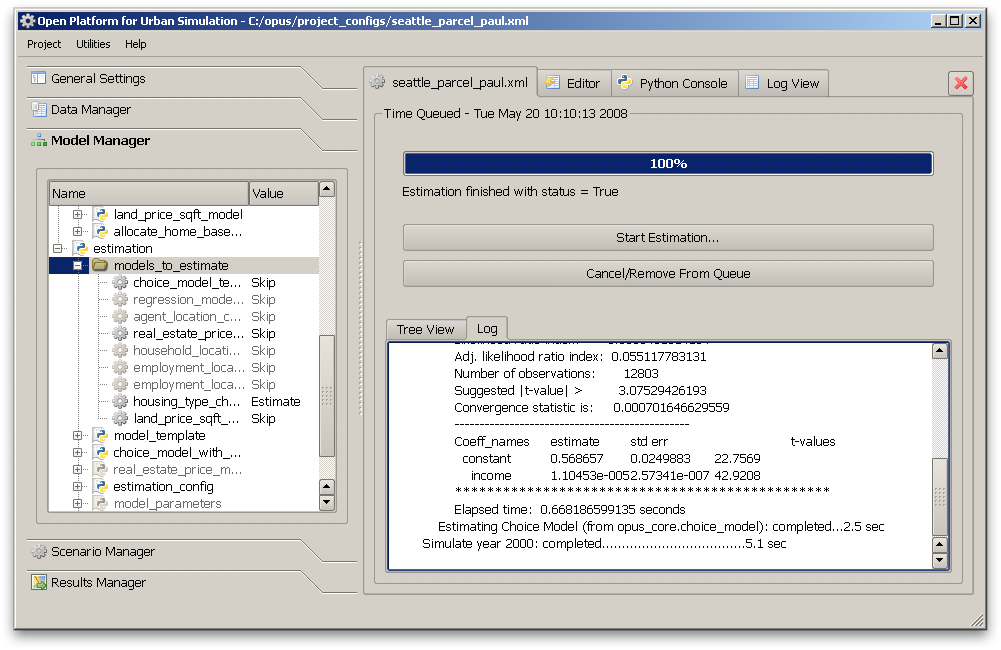
\includegraphics[scale=0.35]{graphics/choice-model-estimation.png}
\end{center}
\caption{Estimating the Housing Type Choice Model}
\label{fig:choice-model-estimation}
\end{figure}
